\documentclass[../mattg_ti-fi_lit-review.tex]{subfiles}

\subsection{\cadmiumtelluride{}/\mercurytelluride{}/\cadmiumtelluride{} quantum wells} \label{sec:ti_mat_hgte_qws}
The \{Hg,Cd\}Te quantum well (QW) was the first successful experiment of a QSH insulator (a 2D TI), with thin layer of \mercurytelluride{} sandwiched between two layers of \cadmiumtelluride{} (Fig. \ref{fig:hgte_schem}).
This system becomes 2D due to quantum confinement from quenching of the out-of-plane direction. 
Bulk \mercurytelluride{} exhibits a band inversion necessary to observe a QSH effect, where as \cadmiumtelluride{} does not. However, \mercurytelluride{} is also a zero-gap semiconductor due to a symmetry protected $\Gamma$ point. By sandwiching \mercurytelluride{} in \cadmiumtelluride{}, the slightly larger lattice parameter of \cadmiumtelluride{} applies a strain on the crystal structure of the thin \mercurytelluride{} when grown the MBE, such that the cubic lattice symmetry is broken and leads to a bandgap opening, becoming a genuine insulator. BHZ predicted that above some critical thickness, the band inversion would be retained and become a TI \cite{bernevig_quantum_2006}.

\begin{figure}[H]
	\centering
	\begin{minipage}[t]{.45\textwidth}
		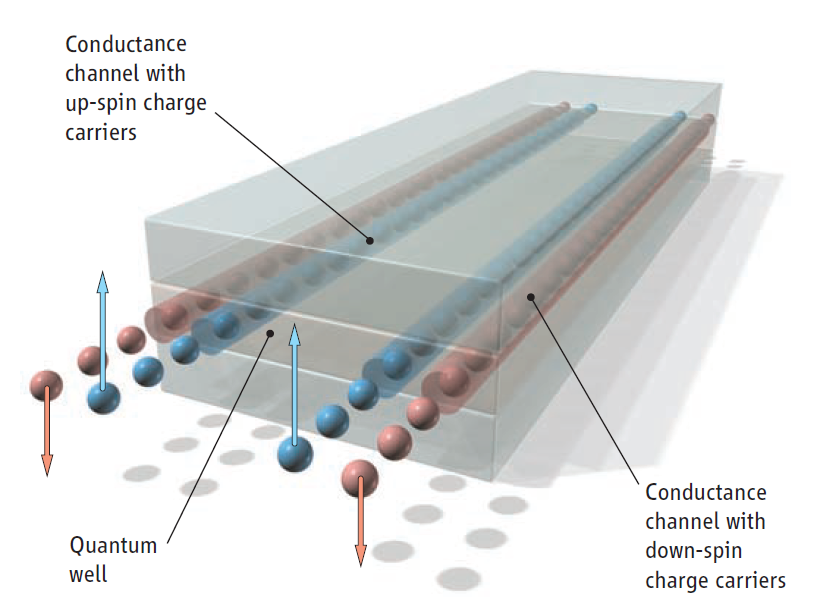
\includegraphics[width=\linewidth]{HgTe_schem}
		\caption{Schematic of \cadmiumtelluride{}/\mercurytelluride{} QW structures. Devices were patterned into hall bar geometries. 
		\\Source: K\"onig \etal{} \cite{konig_quantum_2007}, Science 318}
		\label{fig:hgte_schem}
	\end{minipage}
	\hspace{0.05\textwidth}
	\begin{minipage}[t]{.45\textwidth}
		\includegraphics[width=\linewidth]{HgTe_qshe}
		\caption{The longitudinal four-probe resistance of various \cadmiumtelluride{}/\mercurytelluride{} QW structures. \mercurytelluride{} thickness in I is 5.5nm, II,III and IV are 7.3nm. All devices measured at B=0T, T=30mK.
		\\Source: K\"onig \etal{} \cite{konig_quantum_2007}, Science 318}
		\label{fig:hgte_qsh}
	\end{minipage}
\end{figure}

These characteristics were confirmed later by K\"onig \etal{} \cite{konig_quantum_2007} from the W\"urzburg group, as shown in Fig. \ref{fig:hgte_qsh}. The detected thickness at which the band inversion occurred was at 6.3nm (almost exactly at the prediction of 6.4nm \cite{bernevig_quantum_2006}), where the observation of a quantised conductance became present at low temperatures, previously having diverging resistance. This material only had a bandgap of 10meV resulting from the strain, and so could only be property measured at sufficiently low temperatures. A quick back of the envelope calculation using $k_B T = \Delta E$ gives a temperature of 116.04 K. \newline

\textcolor{orange}{Q: Why was there a lack of band-inversion prior to 6.3nm? As the crystal gets thicker, the less the epitaxial stretching affects the lattice parameters and consequently allows room for band inversion, whilst maintaining a bandgap? If I get too thick, do I just return to \mercurytelluride{} behaviour which has a closed gap?}

\subsection{\bismuthantimony{}}\label{sec:ti_mat_bismuthantimony}

Bismuth Antimony (\bismuthantimony{}) is the first 3D topological insulator discovered \cite{hsieh_topological_2008}, after its prediction well grounded prediction by Fu and Kane \cite{fu_topological_2007-2}. The concentrations for which the alloy \bismuthantimony{} becomes a TI are shown in Fig. \ref{fig:ti_bisb_phases}.

\begin{figure}[H]
	\centering
	\begin{minipage}[t]{.45\textwidth}
		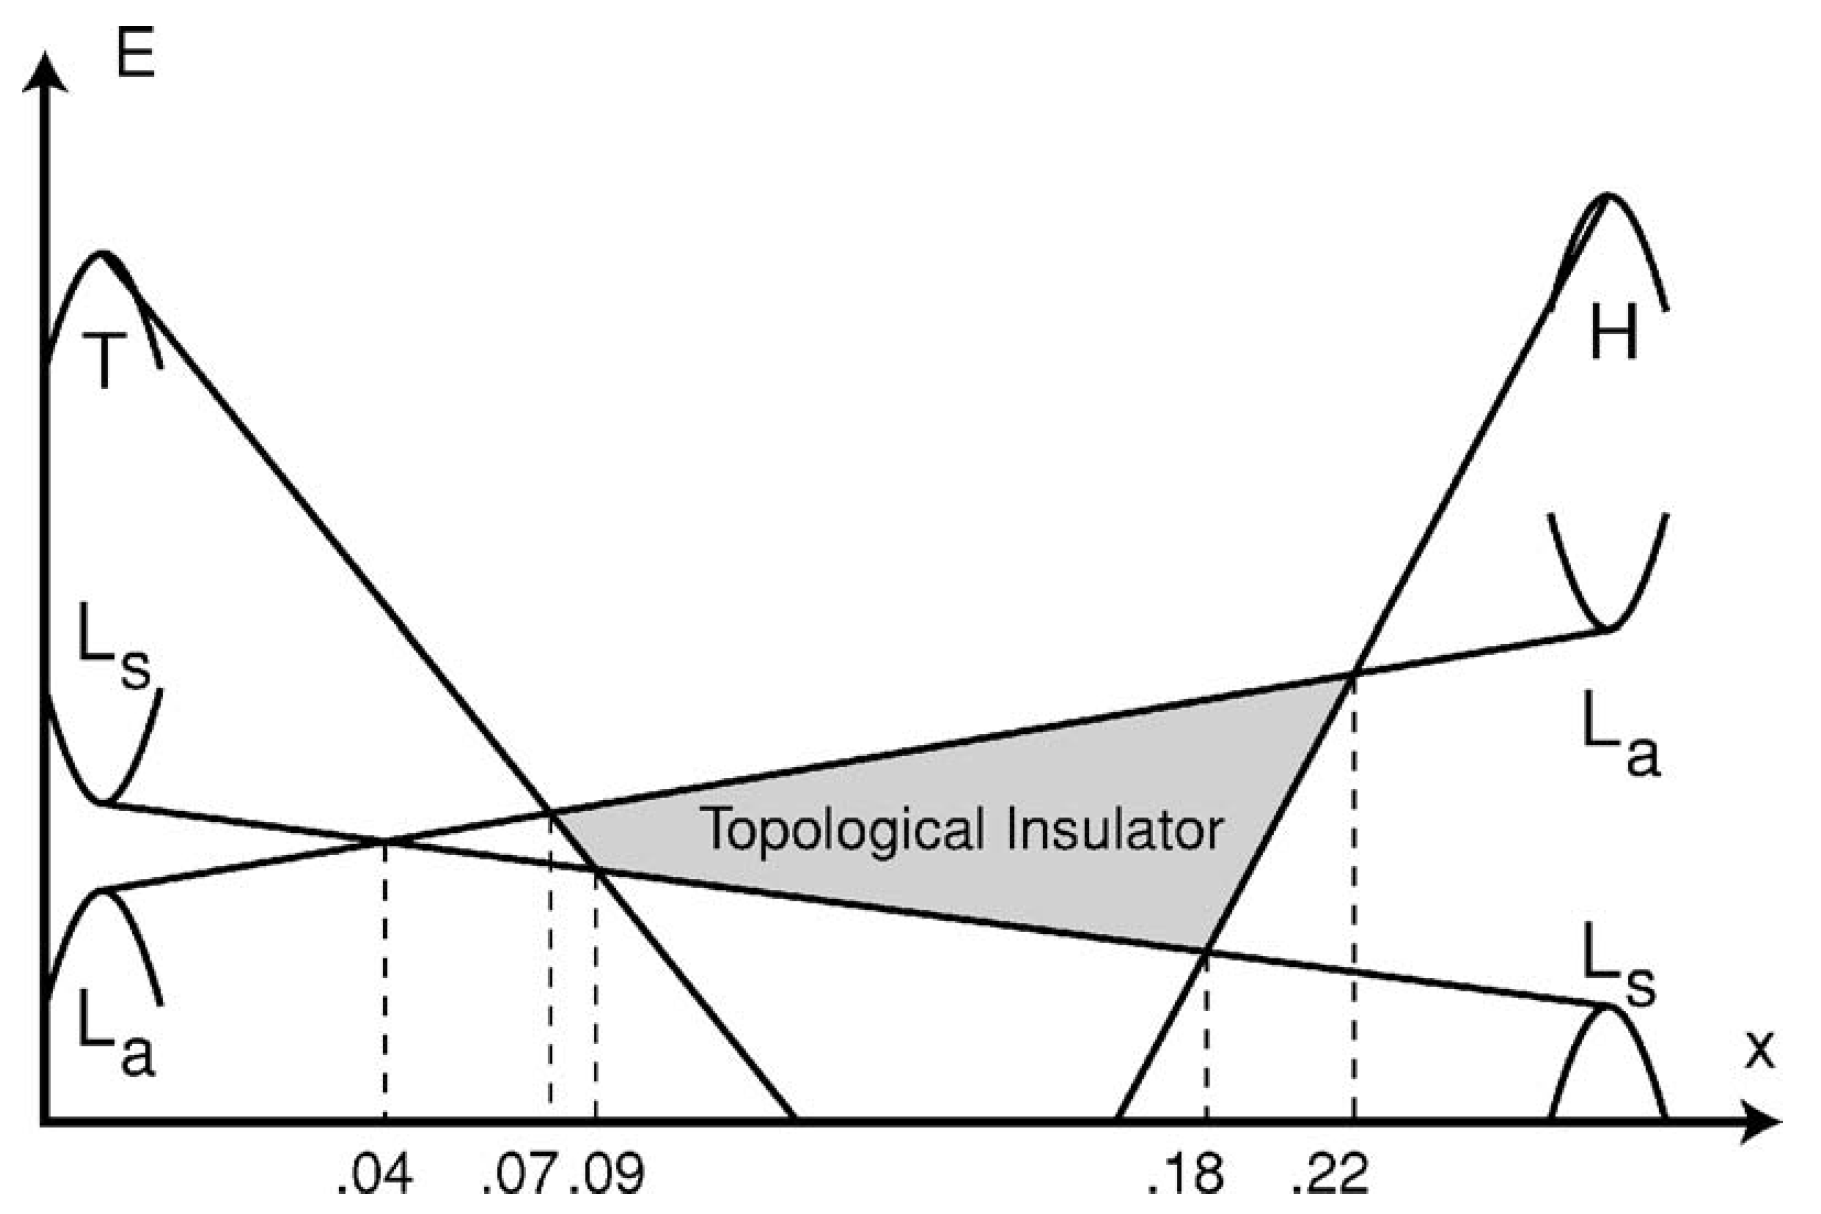
\includegraphics[width=\linewidth]{ti_bisb_phases}
		\caption{The band energy evolution of \bismuthantimony{} as function of the antimony percentage $x$.
		\\Source: Fu and Kane\cite{fu_topological_2007-2}, Phys. Rev. B 76, 045302}
		\label{fig:ti_bisb_phases}
	\end{minipage}
	\hspace{0.05\textwidth}
	\begin{minipage}[t]{.45\textwidth}
		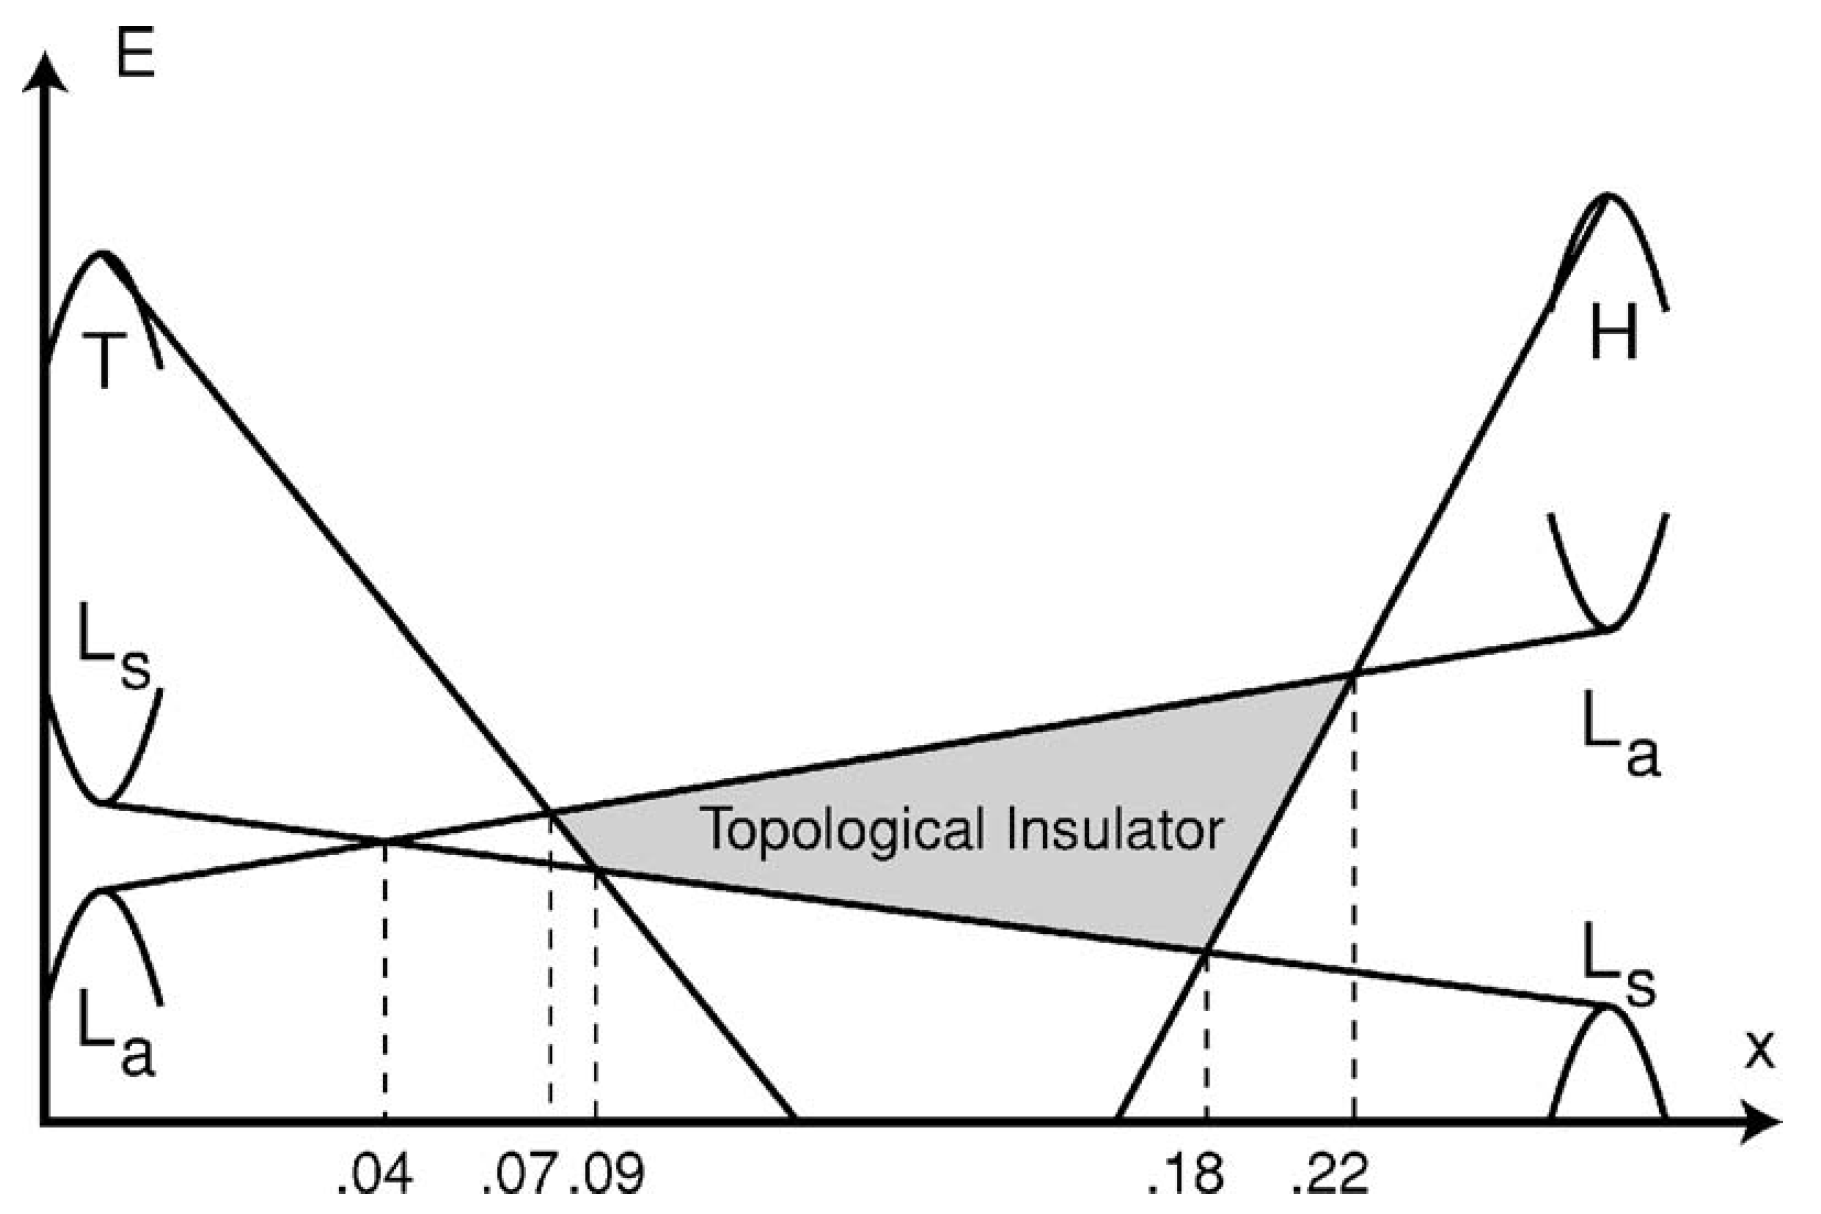
\includegraphics[width=\linewidth]{ti_bisb_phases}
		\caption{
			\\Source: , }
		\label{fig:}
	\end{minipage}
\end{figure}

It is worth noting that \bismuthantimony{} is topologically classed by the \hyperref[sec:z2-3D]{${Z}_2$ 3D invariant} as (1;111).
\bismuthantimony{} boasts a high mobility of $\sim10^4$\mobilityunits, whilst the bulk carrier density can be around $\sim10^{17}$ cm$^{-3}$ \cite{schafgans_landau_2012}. This sort of mobility makes it easy to study 2D quantum transport according to Ando \cite{ando_topological_2013}. 

\textcolor{orange}{High mobility devices useful for studying because?}

Unfortunately, the material's surface states also inherit the strong Rashba-split surface states that are not topological coming from Bismuth; there are 2-4 Fermi-level crossings owing to the Rashba effect, whilst only one topological band (depending on chemical potential), making it complicated to clearly analyse the topological physics present, as discussed in Sec. \ref{sec:ARPES-SR}.


\subsection{\{Bi,Sb\}$_2$\{Se,Te\}$_3$ family}
%\subsection{A$_2$B$_2$B'$_1$ family}
\bismuthtelluride{} was originally suggested as a candidate without band calculations by Fu and Kane \cite{fu_topological_2007-2}. However, Zhang \etal{} \cite{zhang_topological_2009-1} filled in the calculations gap, and additionally predicted a whole family of related structures, generalised by the form $A_2B_2B^\prime_1$. 

These materials form in a rhombohedral crystal structure, containing 26 $A$ atoms, 26 $B$ atoms, and 20 $B^\prime$ atoms, seen in Fig \ref{fig:ti_bi2se3_cryst}a). However, they're named after their stacked structure of \textbf{quintuple layers}, where there are 10 $A$ atoms, 10 $B$ atoms and 5 $B^\prime$ atoms (on average), making a ratio of (2,2,1), or if $B\equiv B^\prime$, (2,3). In the latter case, they are also known as tetradymites.

This class of materials covalently bond within their quintuple layers, but only weakly interact through van der Waals forces, which allows the cleaving between such layers.

\begin{figure}[H]
	\centering
	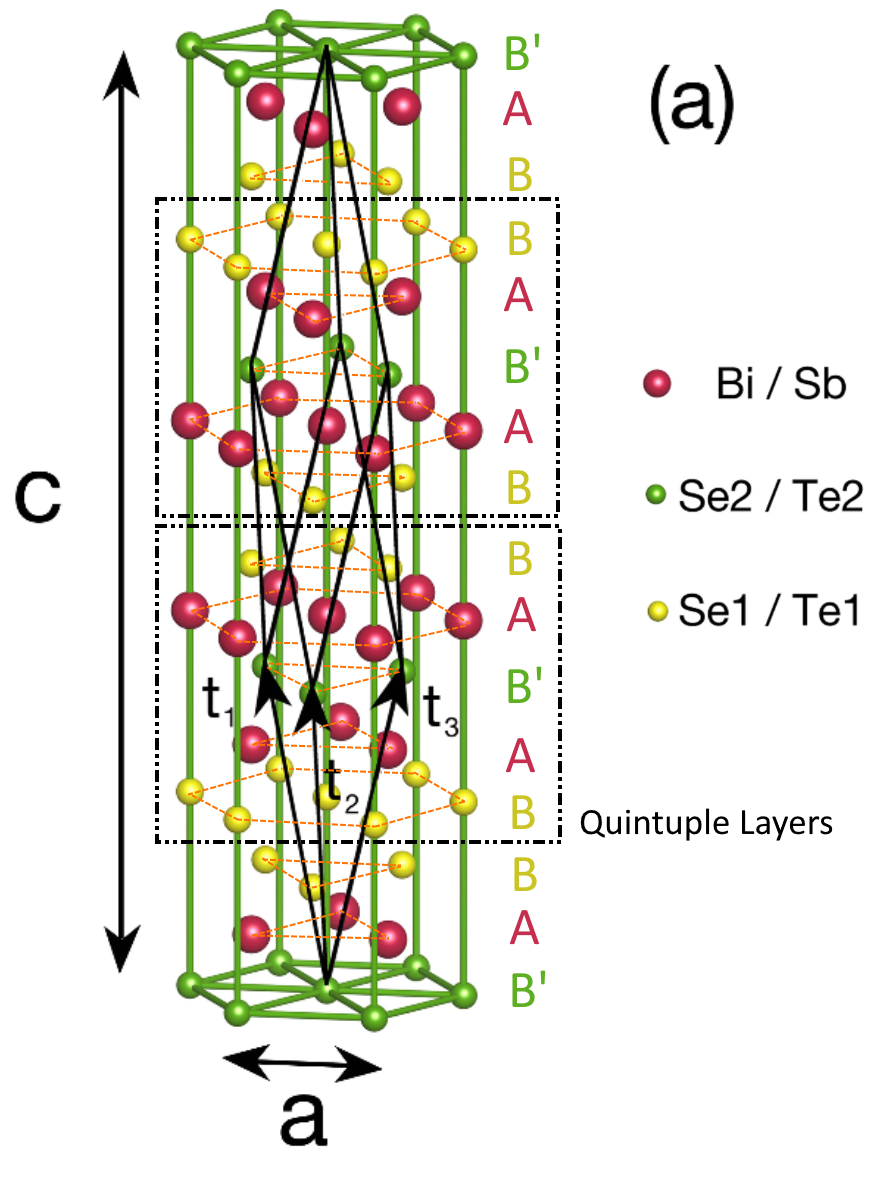
\includegraphics[width=0.45\linewidth]{ti_bi2se3_cryst}
	\hspace{0.05\textwidth}
	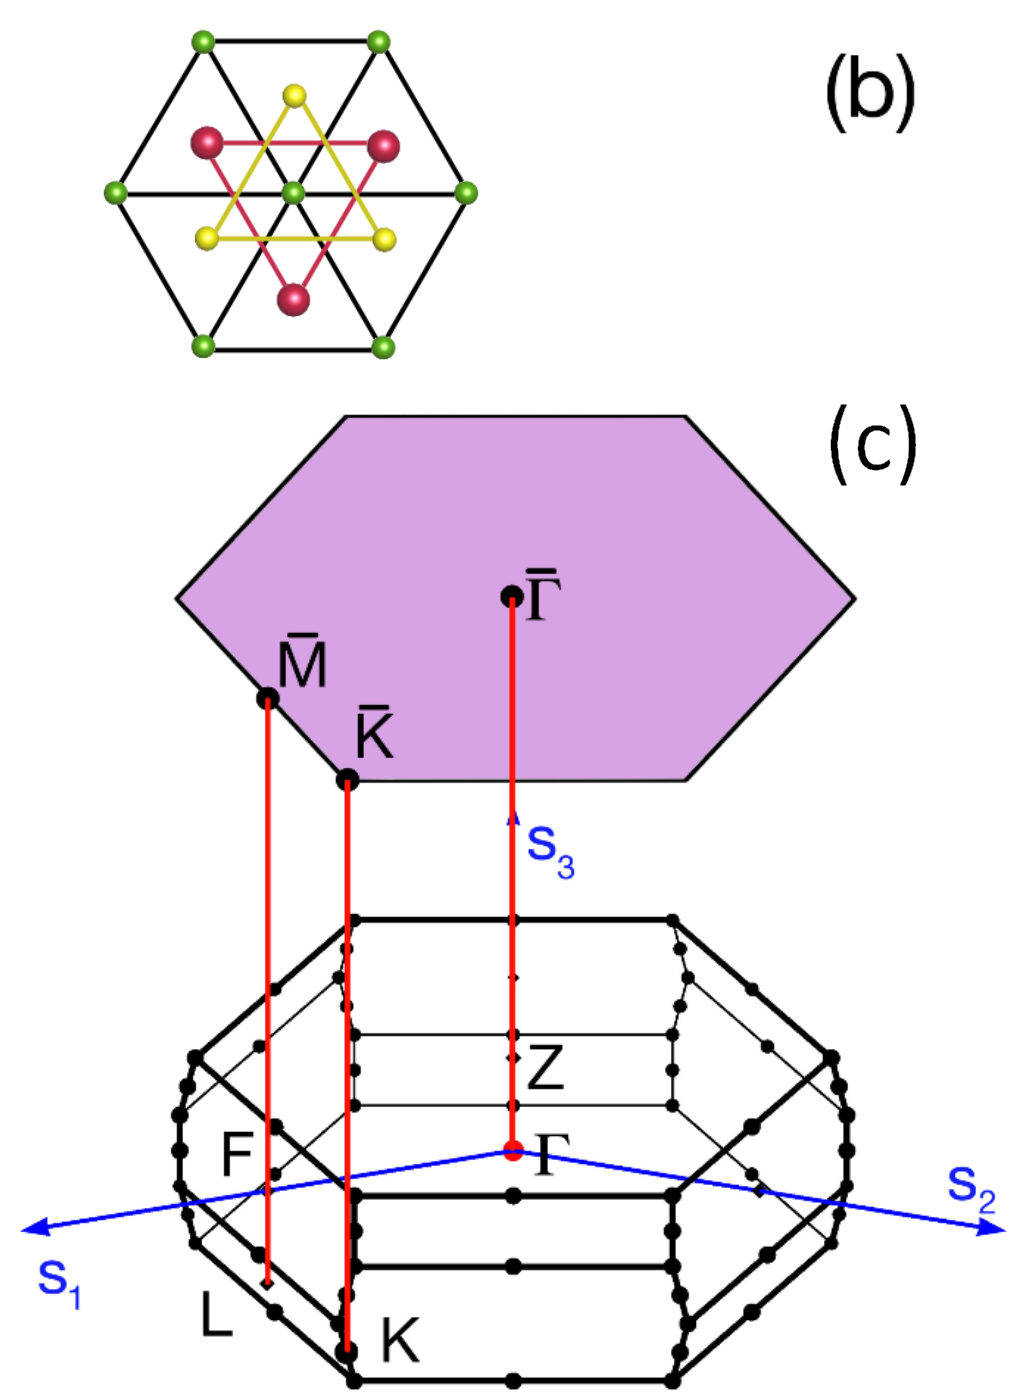
\includegraphics[width=0.45\linewidth]{ti_bi2se3_kspace}
	\caption{A$_2$B$_2$B'$_1$ family. \textbf{a)} Rhombohedral unit cell (c $\sim$ 3 nm). \textbf{b)} Z-axis view of unit cell. \textbf{c)} Bulk Brillouin zone projected along the [111] direction (purple shaded area).
	\\Adapted from: Aramberri and Mu\~noz \cite{aramberri_strain_2017}, Phys. Rev. B 95, 205422 (2017)}
	\label{fig:ti_bi2se3_cryst}
\end{figure}

The tetradymite members of this family include \bismuthtelluride{}, \bismuthselinide{}, and \antimonytelluride{}. Interestingly Zhang's calculations determined \antimonyselenide{} to not be a topological insulator.

Other materials that are tetradymite chalcogenides include \bismuthtellurideselenide{}. 

\subsubsection{\bismuthselinide{}}\label{sec:ti_mat_bi2se3}
The first observation of the Dirac cone in bismuth selenide (\bismuthselinide{}) was reported by Xia \etal{} \cite{xia_observation_2009} Unlike many other topological materials, \bismuthselinide{} is close to the Dirac cone undoped, as shown in Fig. \ref{fig:ti_bi2se3_arpes}. 

In a landmark study, Hsieh \etal{} \cite{hsieh_tunable_2009} observe the first significant evidence of helical Dirac fermions, whilst showing the tunability of \bismuthselinide{} by using a stoichiometric Bi$_{2-\delta}$Ca$_{\delta}$Se$_{3}$.

Normally \bismuthselinide{} is n-type doped due to vacancies or excess selenium \cite{xia_observation_2009} that accumulate through sample growth. It has a bandgap of $\sim 0.35$ eV, 

\begin{figure}[H]
	\centering
	\begin{minipage}[t]{.45\textwidth}
		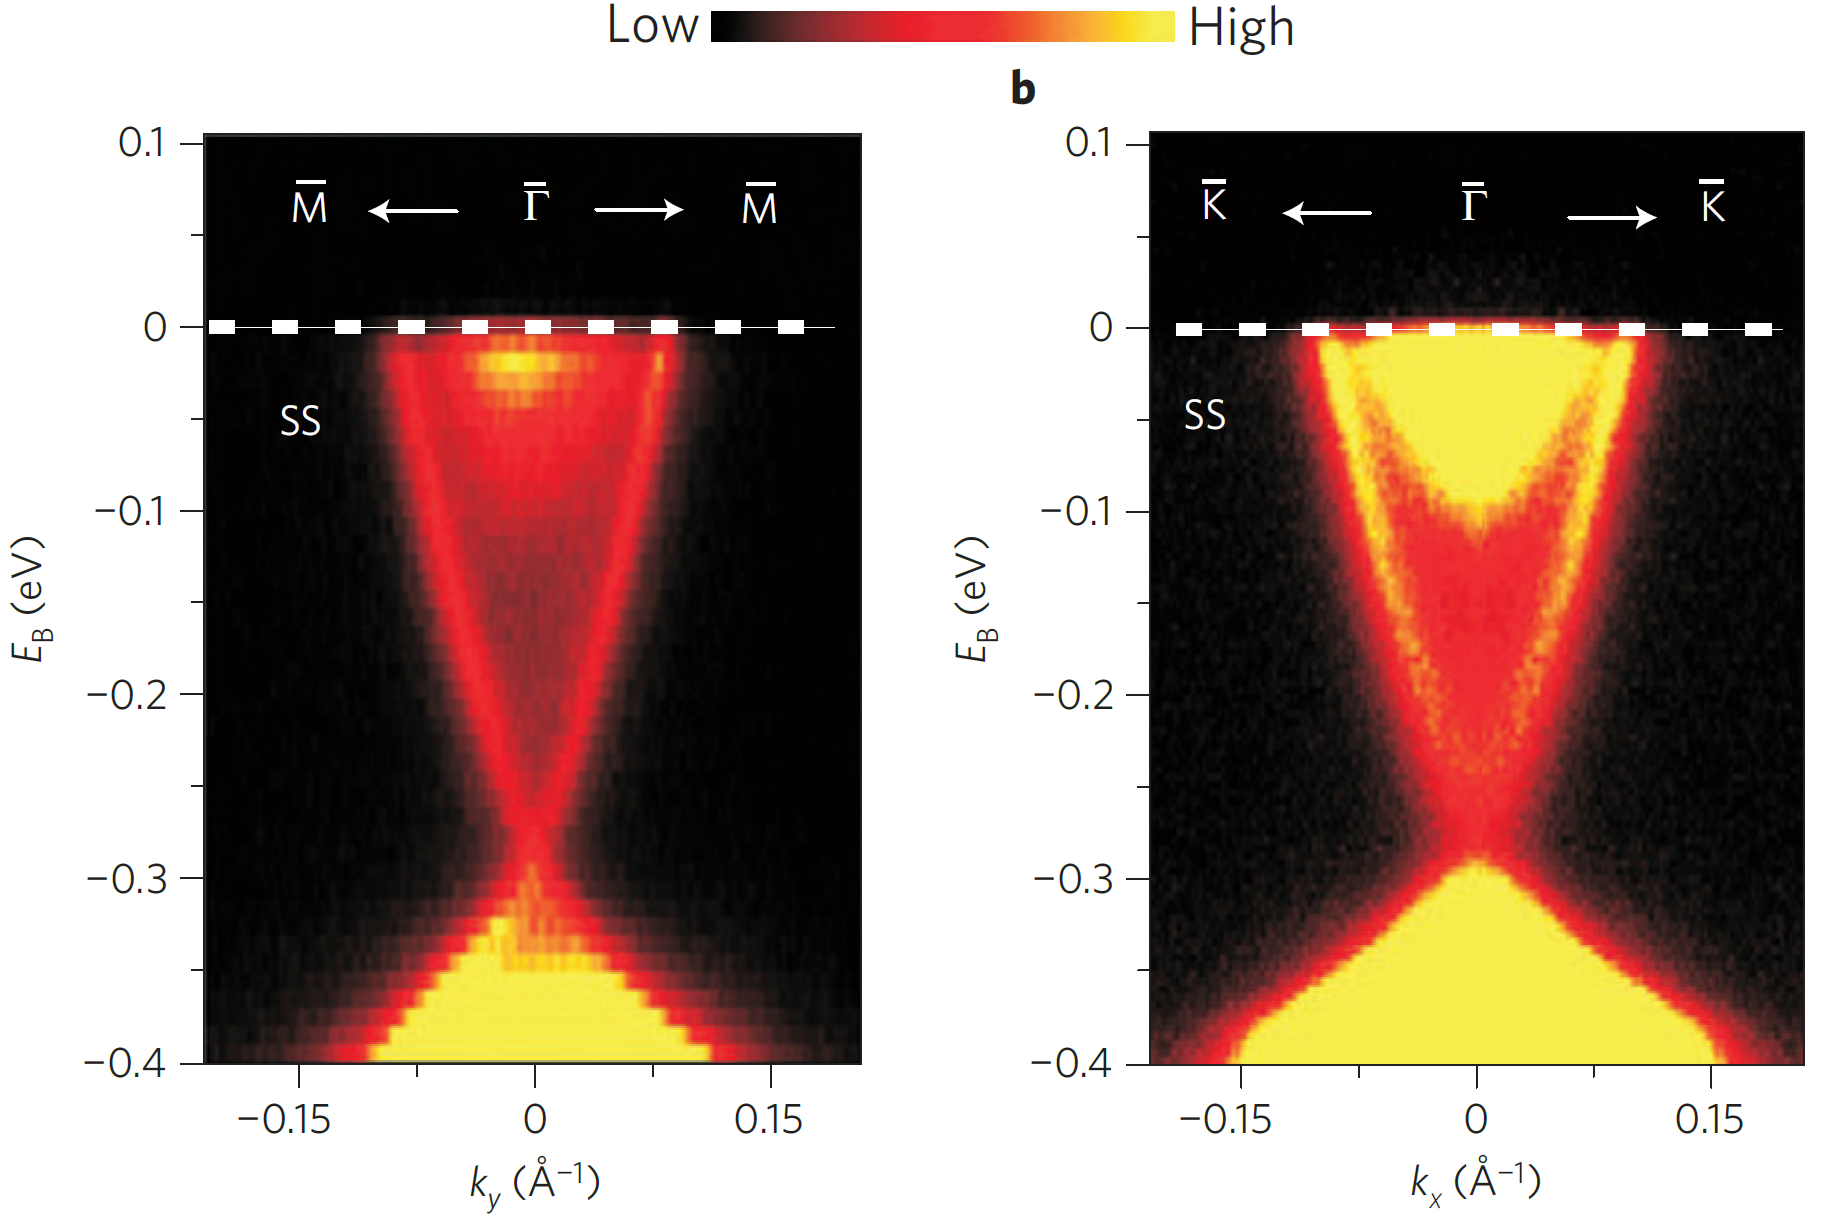
\includegraphics[width=\linewidth]{ti_bi2se3_arpes}
		\caption{ARPES of \bismuthselinide{}. \textbf{a)} From $\Gamma\to M$ \textbf{b)} From $\Gamma \to K$
			\\Source: Xia \etal{} Nature Physics 398, Vol 5 (2009)}
		\label{fig:ti_bi2se3_arpes}
	\end{minipage}
	\hspace{0.05\textwidth}
	\begin{minipage}[t]{.45\textwidth}
	\end{minipage}
\end{figure}

\begin{figure}[H]
	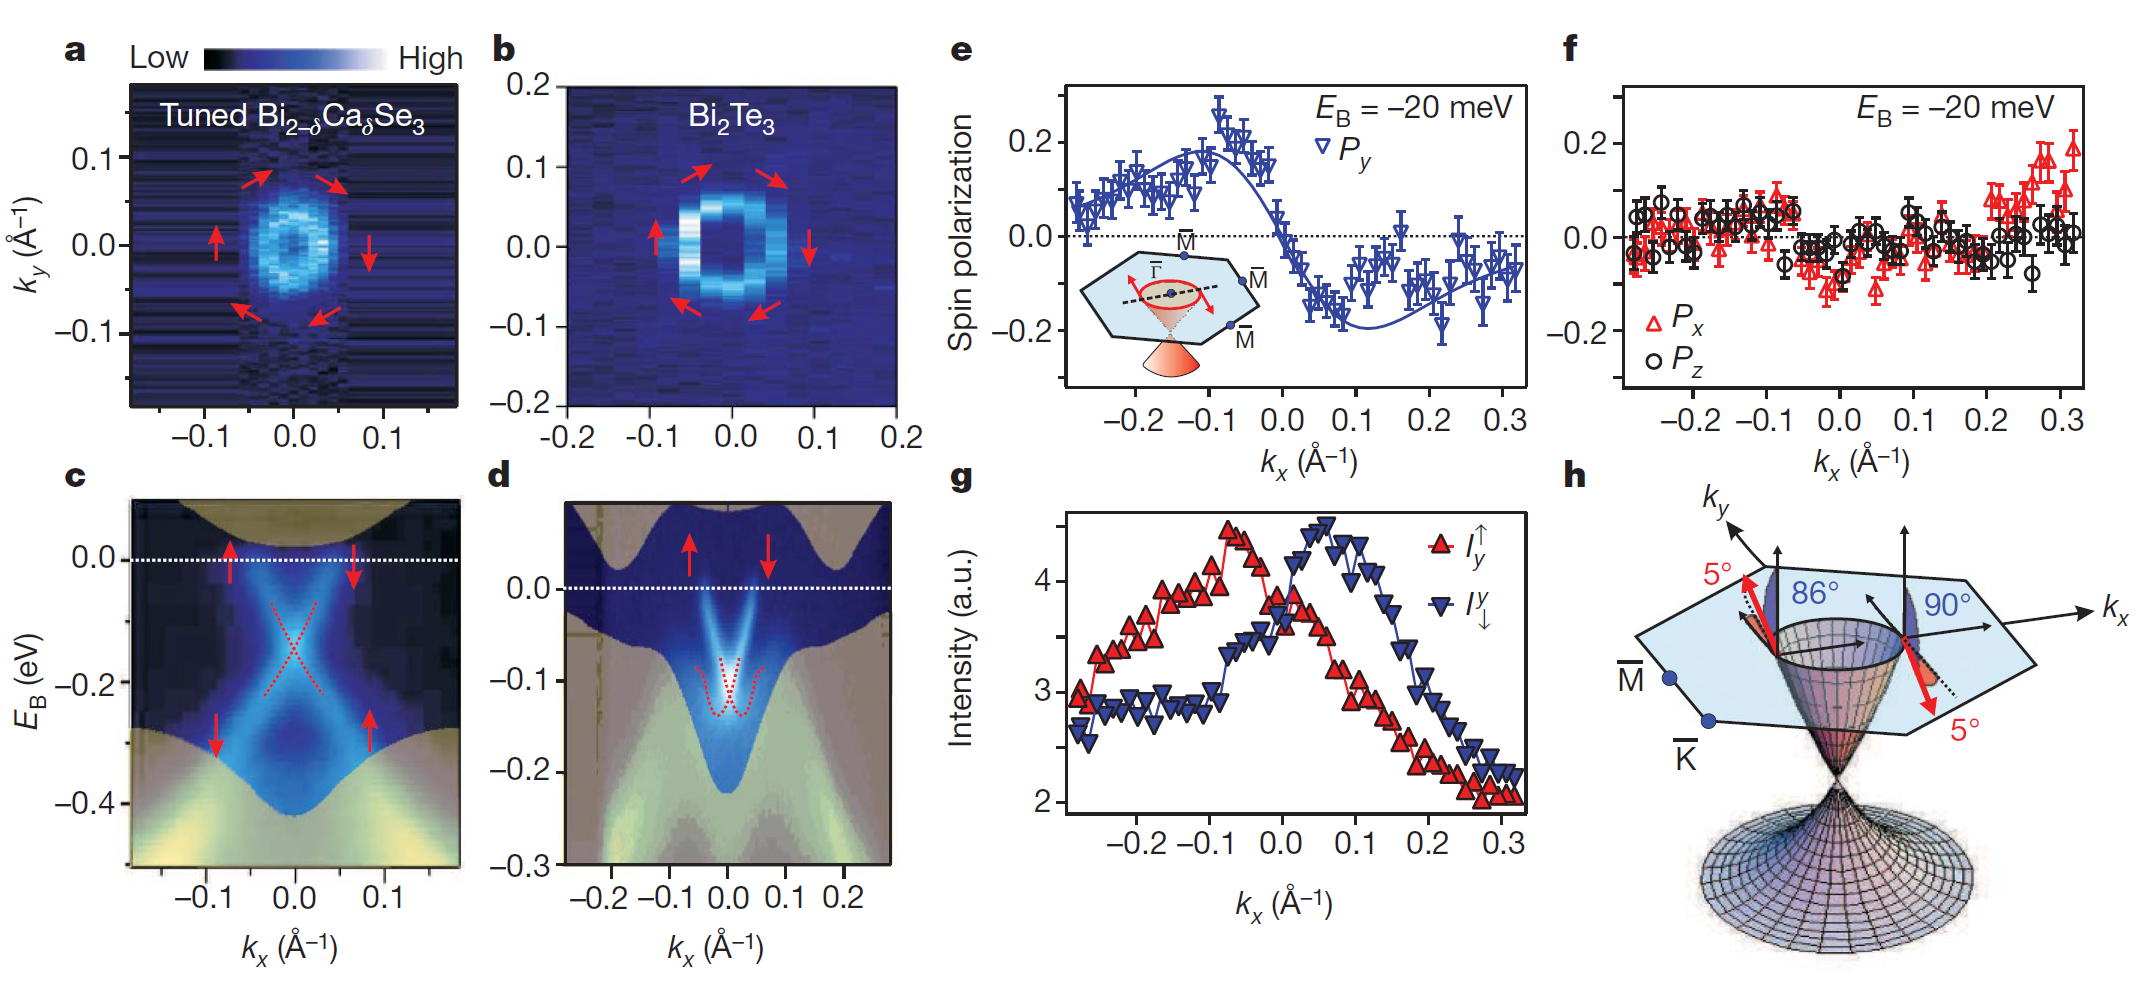
\includegraphics[width=\linewidth]{ti_bi2se3_helical}
	\caption{ \textbf{a,b)} ARPES intensity map of $E_F$ on (111) surface of \textbf{a} Bi$_{2-\delta}$Ca$_{\delta}$Se$_{3}$ and \textbf{b} \bismuthtelluride{}. \\
	\textbf{c,d)} Respective ARPES dispersions along the $k_x$ cut. Yellow shaded reigons are projections of bulk bands of pure \bismuthselinide{} and \bismuthtelluride{}.
	\textbf{e,f)} y component and \{x,z\} components (triangles, circles) of spin polarisation along the $\Gamma$ - $M$ direction, respectively.
	\textbf{}
		\\Source: Hsieh \etal{} Nature 1101, 460 (2009)}
	\label{fig:ti_bi2se3_helical}
\end{figure}


Kim \etal{}\cite{kim_surface_2012} - Observation of zero hall coefficient at the Dirac point - rather than divergence with lack of carriers.
\begin{equation}
R_H = \frac{E_y}{j_x B_z}
\end{equation}



\subsubsection{\bismuthtelluride{}}\label{sec:ti_mat_bi2te3}

\subsubsection{}

%TODO Thermoelectric Materials & SOC effects.
%\subsection{Ties to thermoelectric materials
